\section{VoLTE抓包结果分析}
\label{chap:analyze:results}

%通过抓包测试,得到了一些VoLTE视频流结果
在设计检测方法前,首先构造参照数据集。以三星A5108手机为平台,在多种网络场景下进行视频通话测试,并通过tcpdump抓包软件\nupcite{10.5555/1047846.1047873},捕获所有的视频数据包。

%分析抓包结果,对特征进行分析
\insertTable{
	\begin{table}[htbp]
        \centering
        \caption{VoLTE视频通话抓包结果}
        \label{tab:3:capture-results}
        \begin{threeparttable}
            \begin{tabular*}{0.8\textwidth}{@{\extracolsep{\fill}}ccccc}
            \toprule
            场景 & 通话次数 & 数据包总数 & 抓包总数 & 平均丢包率 \\ 
            \midrule
            Excellent & 13 & 323297 & 320990 & 0.71\% \\ 
            Good & 17 & 288592 & 261470 & 9.4\% \\
            \bottomrule
            \end{tabular*}
            \begin{tablenotes}
                \footnotesize
                \item[] 视频数据包发送速率,约为100\ pkts/s
            \end{tablenotes}
        \end{threeparttable}
    \end{table}
}
如表\nref{tab:3:capture-results},抓包数据由两种场景中获取。Excellent场景对应的是同基站内通话,网络环境稳定;Good场景对应的是跨基站状态下的通话,网络噪声较强。Excellent场景中,通话质量及流畅度极佳,丢包率较低;Good场景中,偶尔存在卡顿或图像模糊,丢包率较高。在两种测试场景中,丢包率不同导致统计分布出现明显差异,检测过程需要分别进行。

\subsection{丢包率}
\label{chap:analyze:results:plr}

%统计的各个通话的全局丢包率,分布情况
\insertFigure{
	\begin{figure}[htbp]
		\centering
        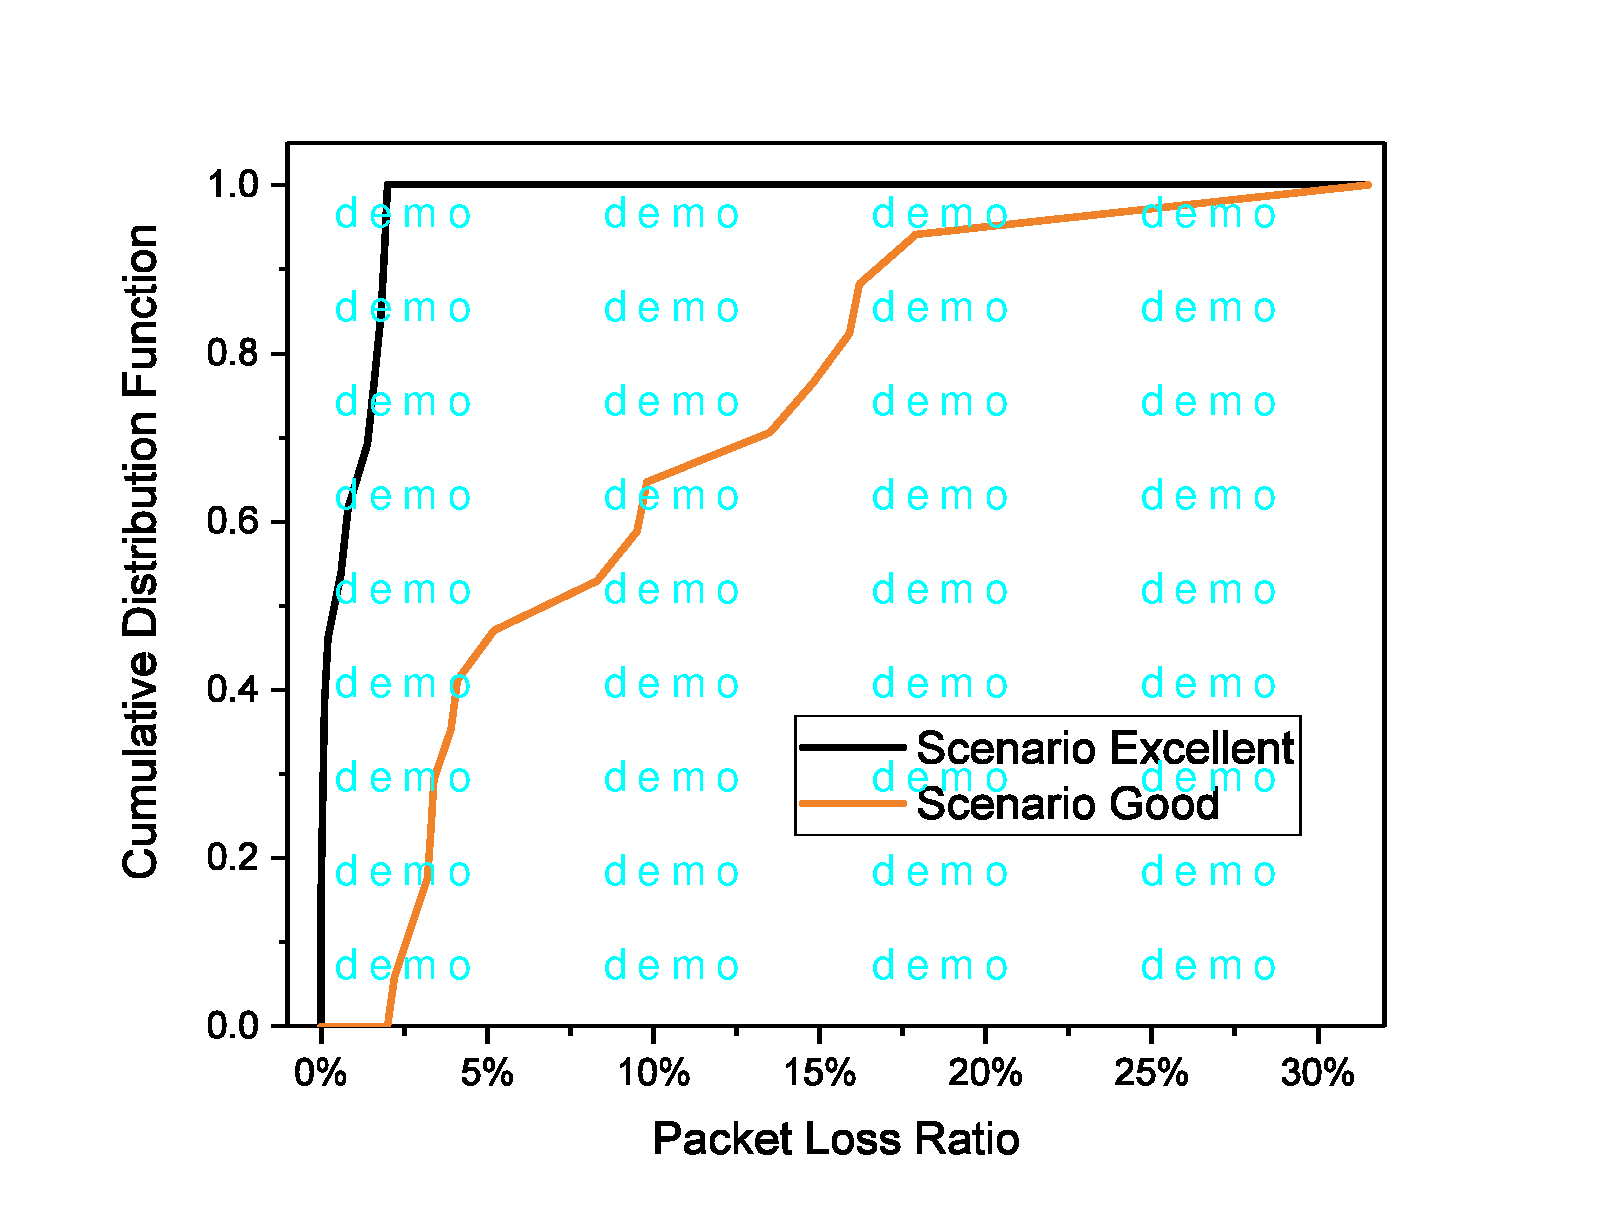
\includegraphics[width=0.7\textwidth]{chapters/chapter3/figures/capture-cdf-plr.pdf}
        \caption{两种场景中平均丢包率的累积分布图}\label{fig:3:cdf-plr}
	\end{figure}
}

如图\nref{fig:3:cdf-plr},两种场景中平均丢包率的累积分布出现明显偏离。Excellent场景下丢包率普遍较低,对时间隐通道的存在更敏感;Good场景中噪声干扰严重,丢包率显著上升,时间隐通道的检测难度增大。

\subsection{区间丢包数}
\label{chap:analyze:results:window}

\insertFigure{
	\begin{figure}[htbp]
		\centering
        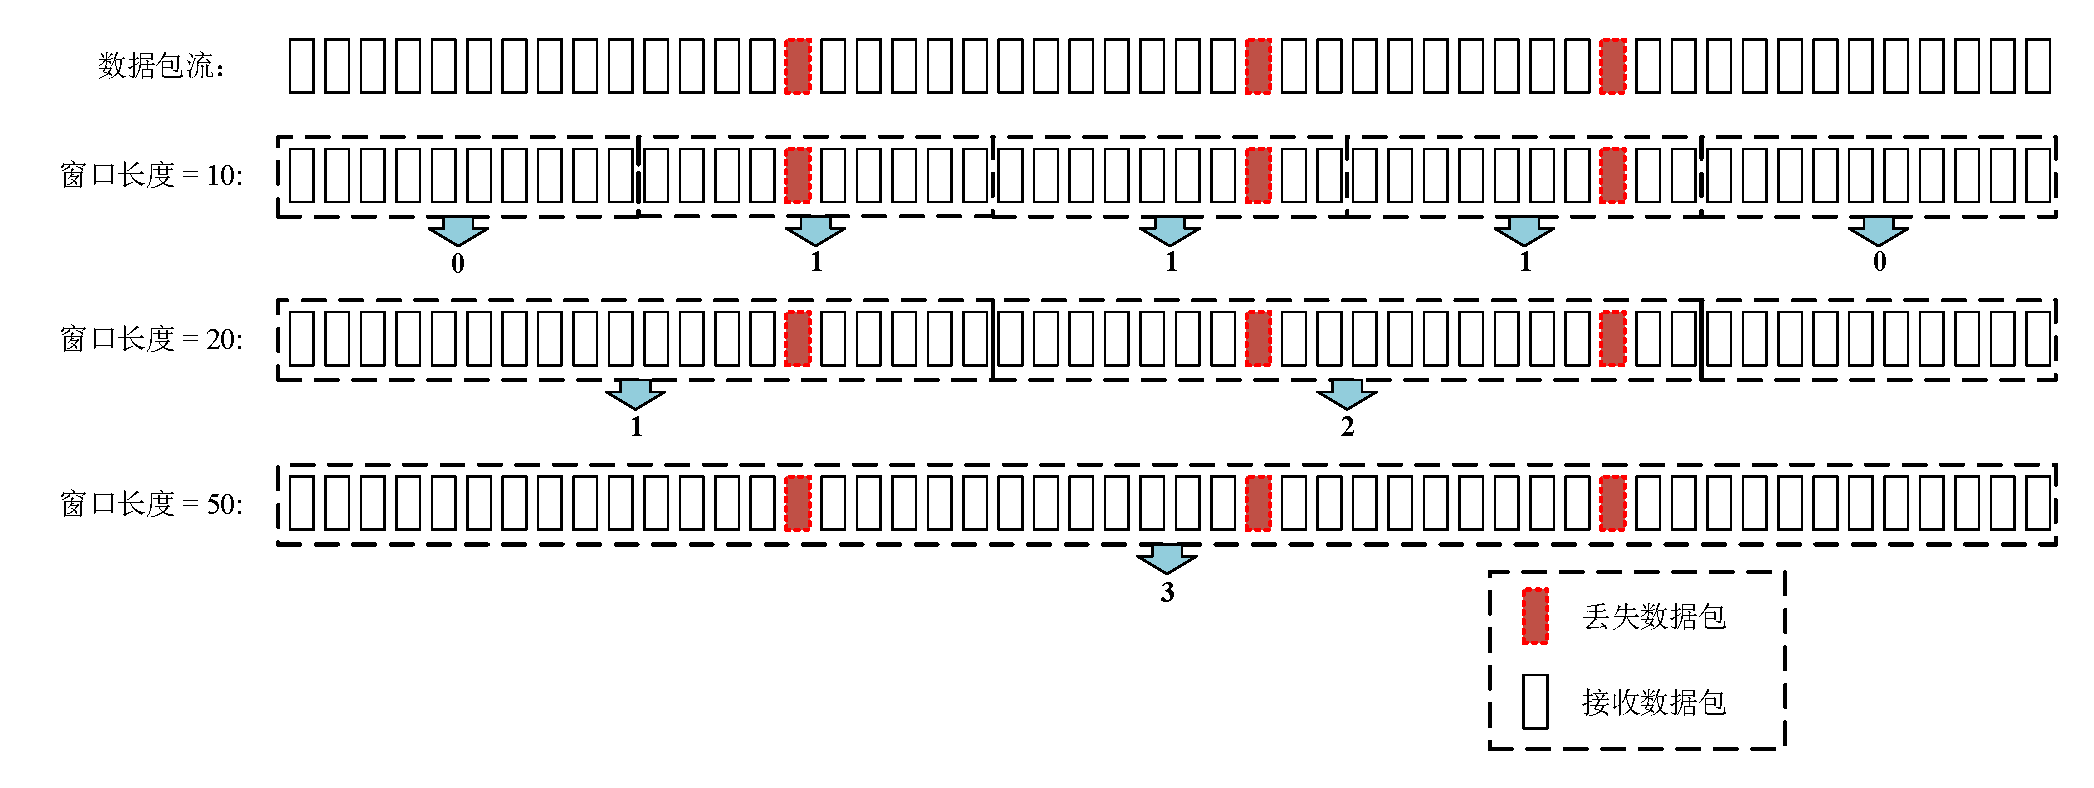
\includegraphics[width=0.99\textwidth]{chapters/chapter3/figures/win-size-count.pdf}
        \caption{窗口大小与区间丢包数示意图}\label{fig:3:win-size-count}
    \end{figure}
}

%测试区间设定,以及不同场景下,各个区间的分布函数
基于区间丢包数的检测方法,首先将数据包按照设定的窗口大小划为独立区间,每个区间内单独统计丢包数量。最终对各区间的统计结果汇总,计算累积分布。如图\nref{fig:3:win-size-count},在相同丢包分布下,通过控制窗口的大小,区间内丢包数量随着窗口增大而累积增加。

\insertFigure{
    \begin{figure}[htbp]
    \centering
        \subfigure[Excellent场景的累积分布函数]{
            \label{fig:3:capture:win-cdf:excellent}
            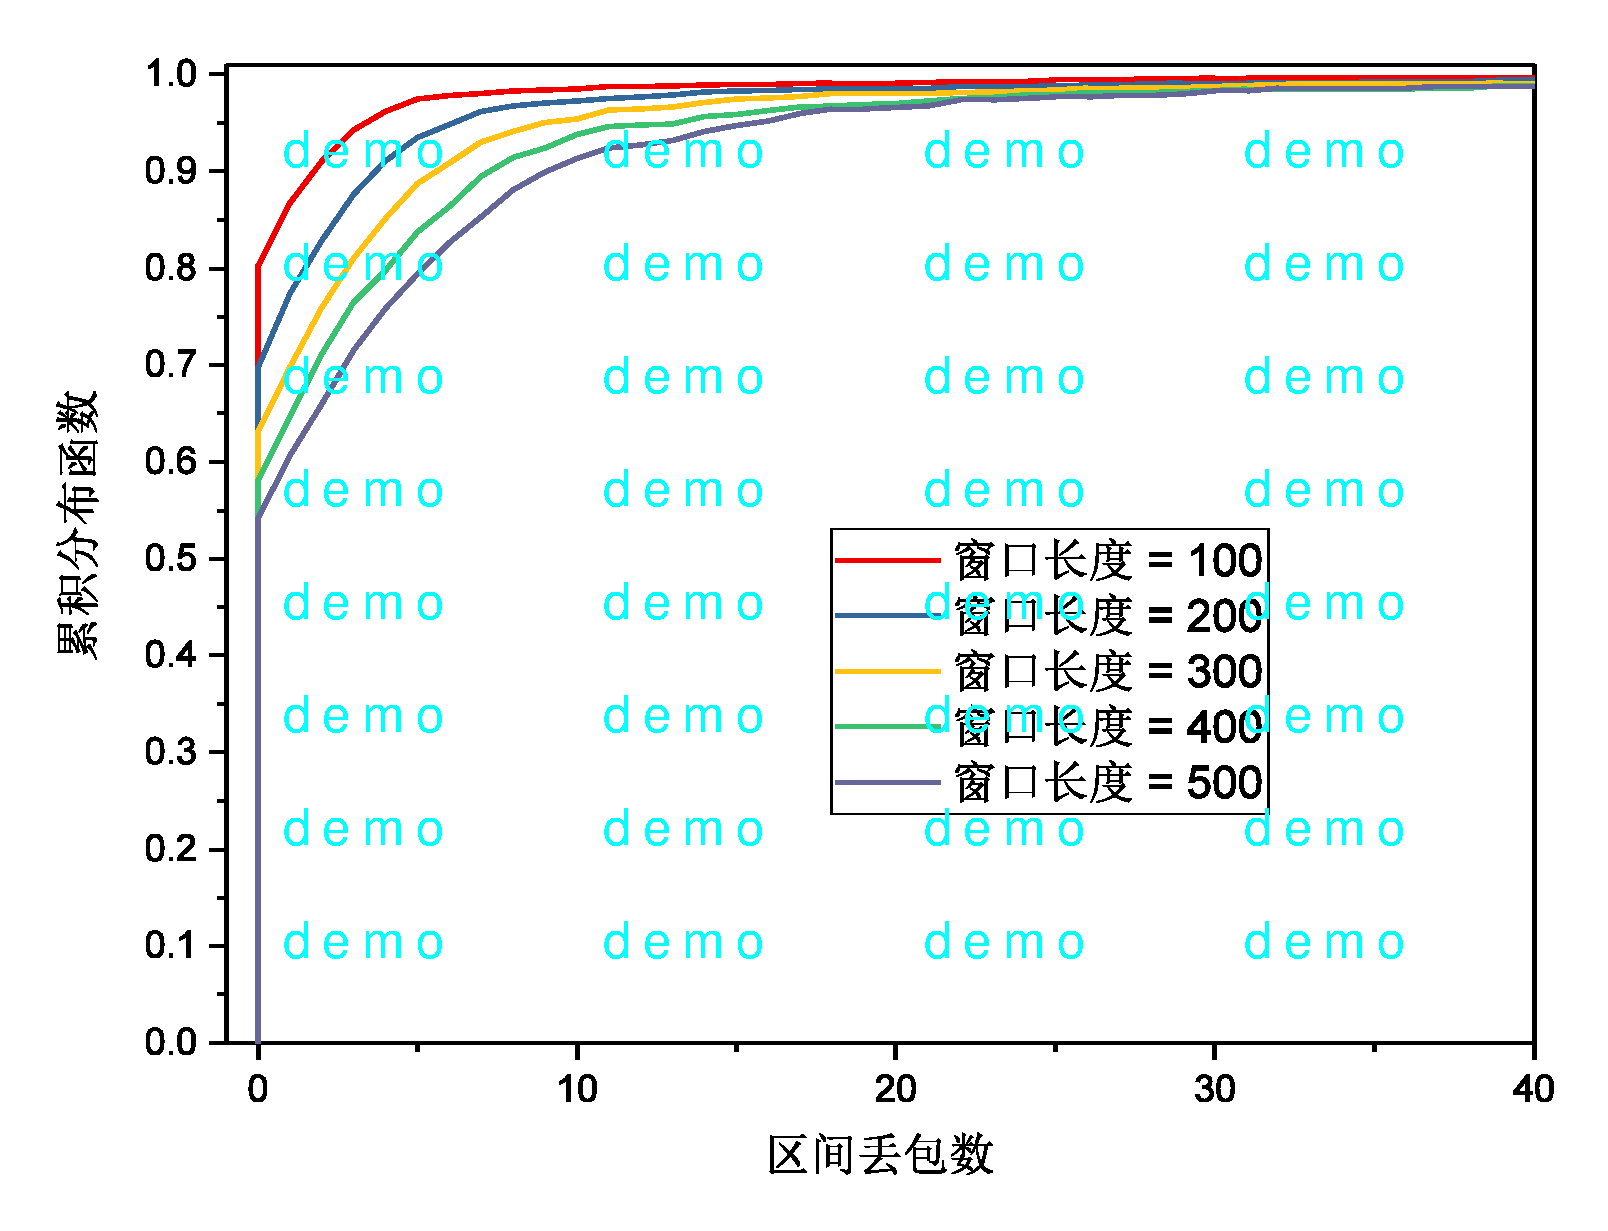
\includegraphics[width=0.48\textwidth]{chapters/chapter3/figures/capture-cdf-win-excellent.pdf}
        }
        \subfigure[Good场景的累积分布函数]{
            \label{fig:3:capture:win-cdf:good}
            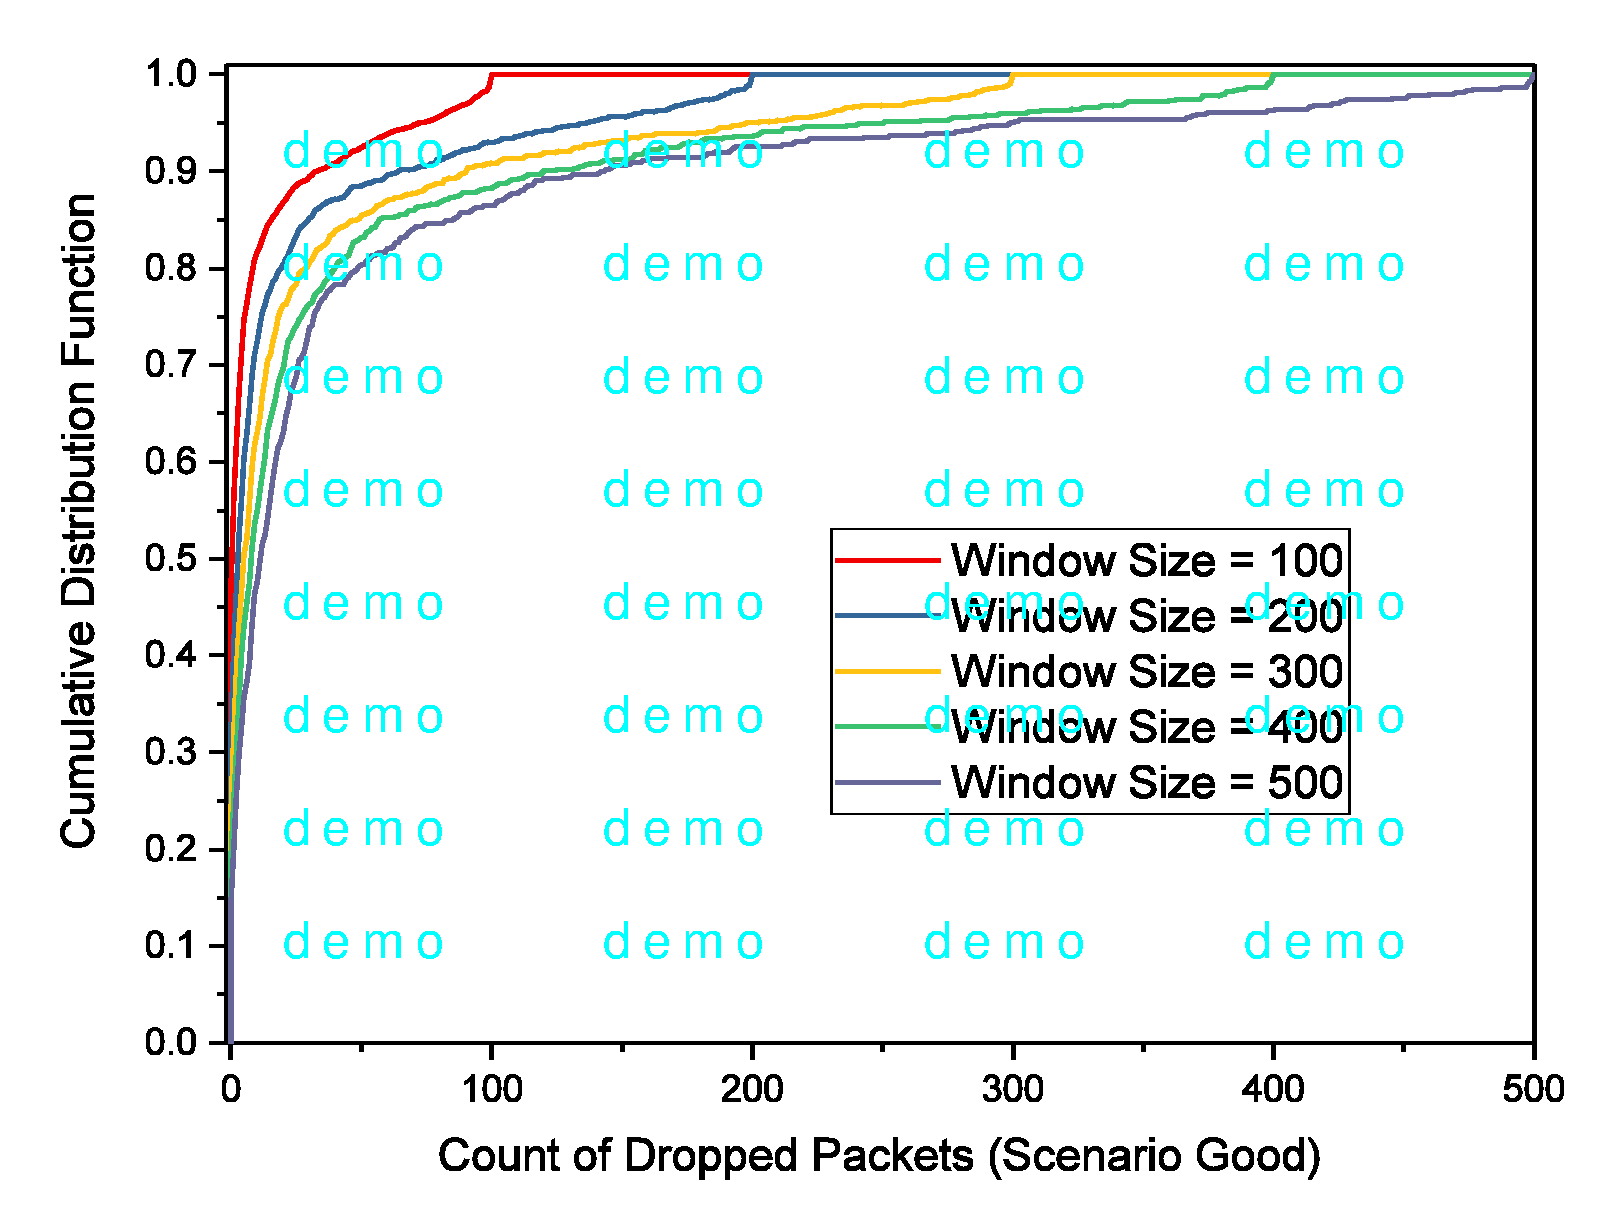
\includegraphics[width=0.48\textwidth]{chapters/chapter3/figures/capture-cdf-win-good.pdf}
        }
    \caption{不同场景区间丢包数的累积分布函数}
    \label{fig:3:capture:win-cdf}
    \end{figure}
}

如图\nref{fig:3:capture:win-cdf},两种场景下的累积分布函数既存在总体相似性,又在存在局部特征的差异。图\nref{fig:3:capture:win-cdf:excellent}中,丢包数量为0的区间均占据一半以上,并且CDF收敛到$1.0$的趋势明显,反应出网络质量极佳。图\nref{fig:3:capture:win-cdf:good}中,曲线上升趋势与图\nref{fig:3:capture:win-cdf:excellent}类似,但丢包数量为0的部分比重较小,并且存在数据包全丢的区间。

\insertFigure{
    \begin{figure}[htbp]
        \centering
            \subfigure[窗口长度200时的概率质量函数]{
                \label{fig:3:capture:win-pmf:200}
                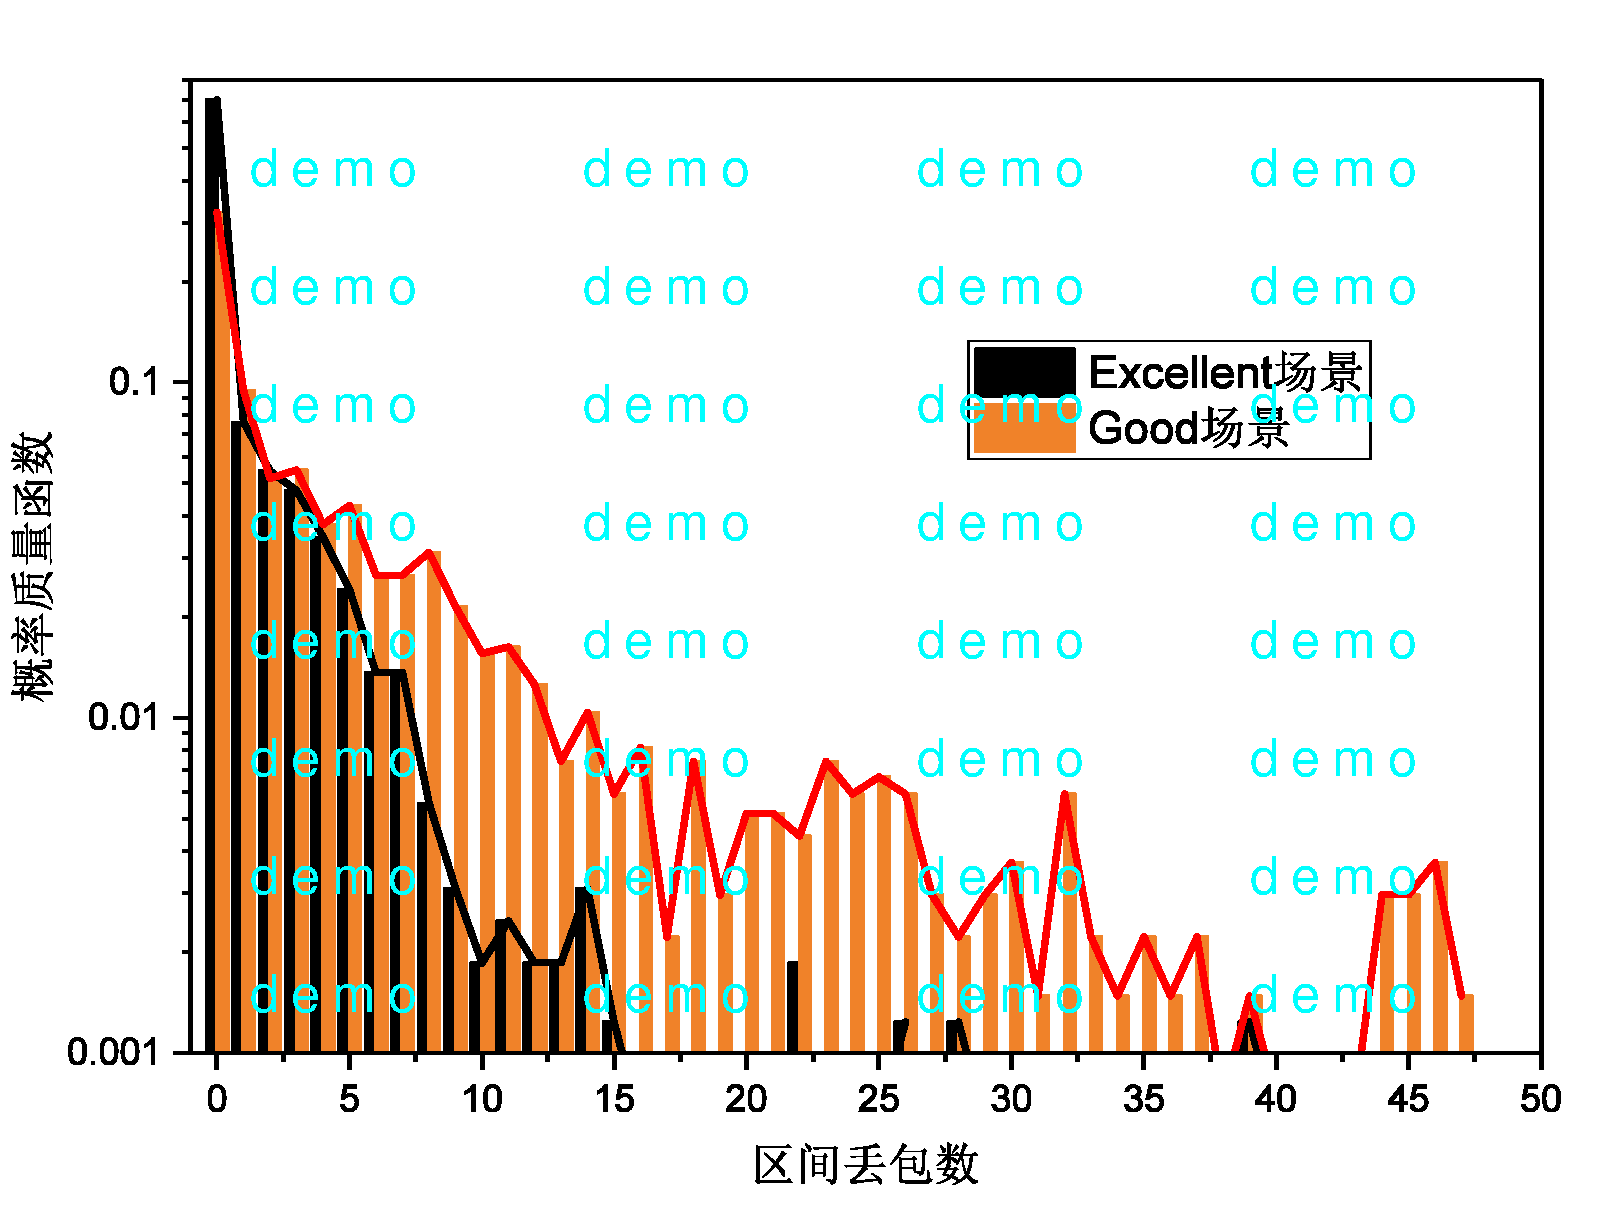
\includegraphics[width=0.48\textwidth]{chapters/chapter3/figures/capture-pmf-win200.pdf}
            }
            \subfigure[窗口长度400时的概率质量函数]{
                \label{fig:3:capture:win-pmf:400}
                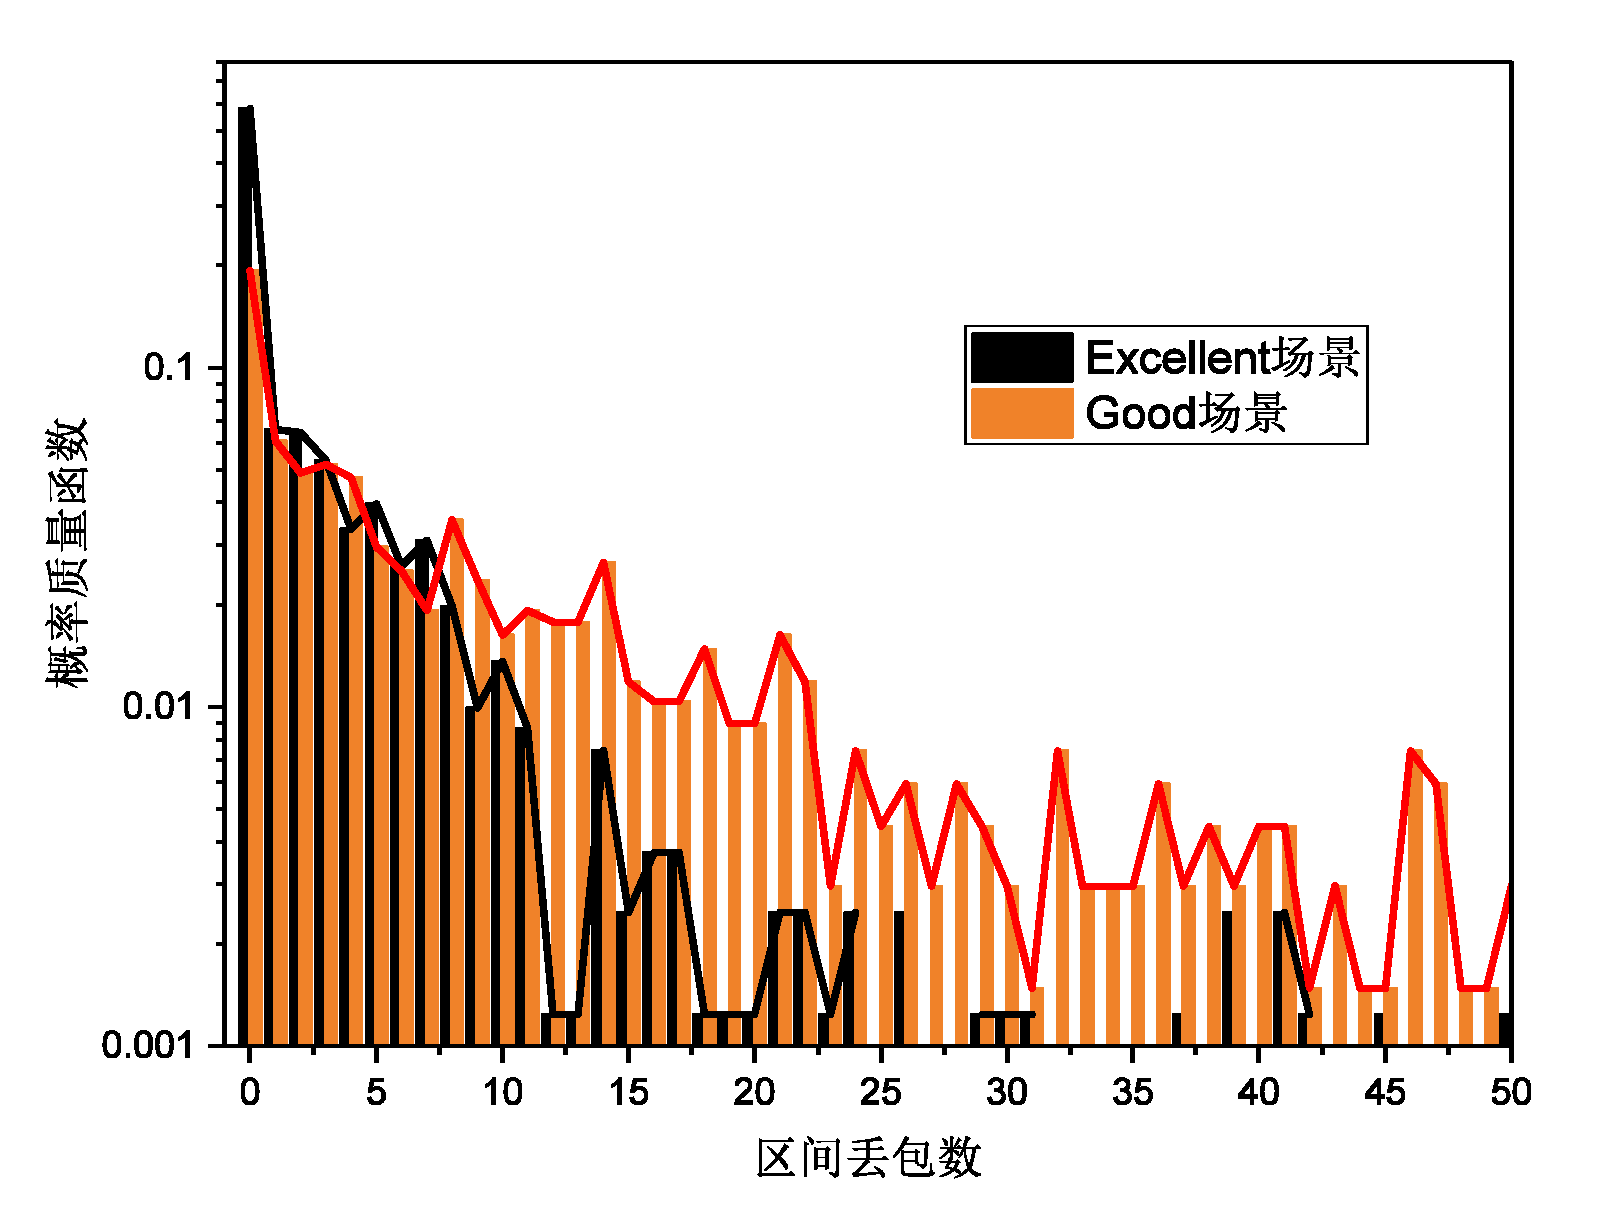
\includegraphics[width=0.48\textwidth]{chapters/chapter3/figures/capture-pmf-win400.pdf}
            }
        \caption{不同场景区间丢包数的概率质量函数}
        \label{fig:3:capture:win-pmf}
        \end{figure}
}

如图\nref{fig:3:capture:win-pmf},不同窗口大小的概率质量函数,在不同的场景中存在显著差异。区间丢包数的概率质量函数变化趋势存在波动,并且在不同场景中变化趋势差距较大,因此对区间丢包数的检验需要从整体的角度进行。

\subsection{数据包传输间隔}
\label{chap:analyze:results:ipd}

%IPD代表了什么
IPD分布是时间隐通道的经典测试对象,如图\nref{fig:2:cdf-ipd},发送阶段的IPD与接收阶段的分布存在明显差异。发送阶段有两个集中分布的区间,而接收阶段曲线变为平滑,证明网络缓冲及数据包转发削弱了原始IPD特征,接收方观测到的IPD接近正偏态分布。

%两种场景下抓包得到的IPD分布
\insertFigure{
    \begin{figure}[htbp]
    \centering
        \subfigure[IPD分布的累积分布函数图]{
            \label{fig:3:capture:ipd:cdf}
            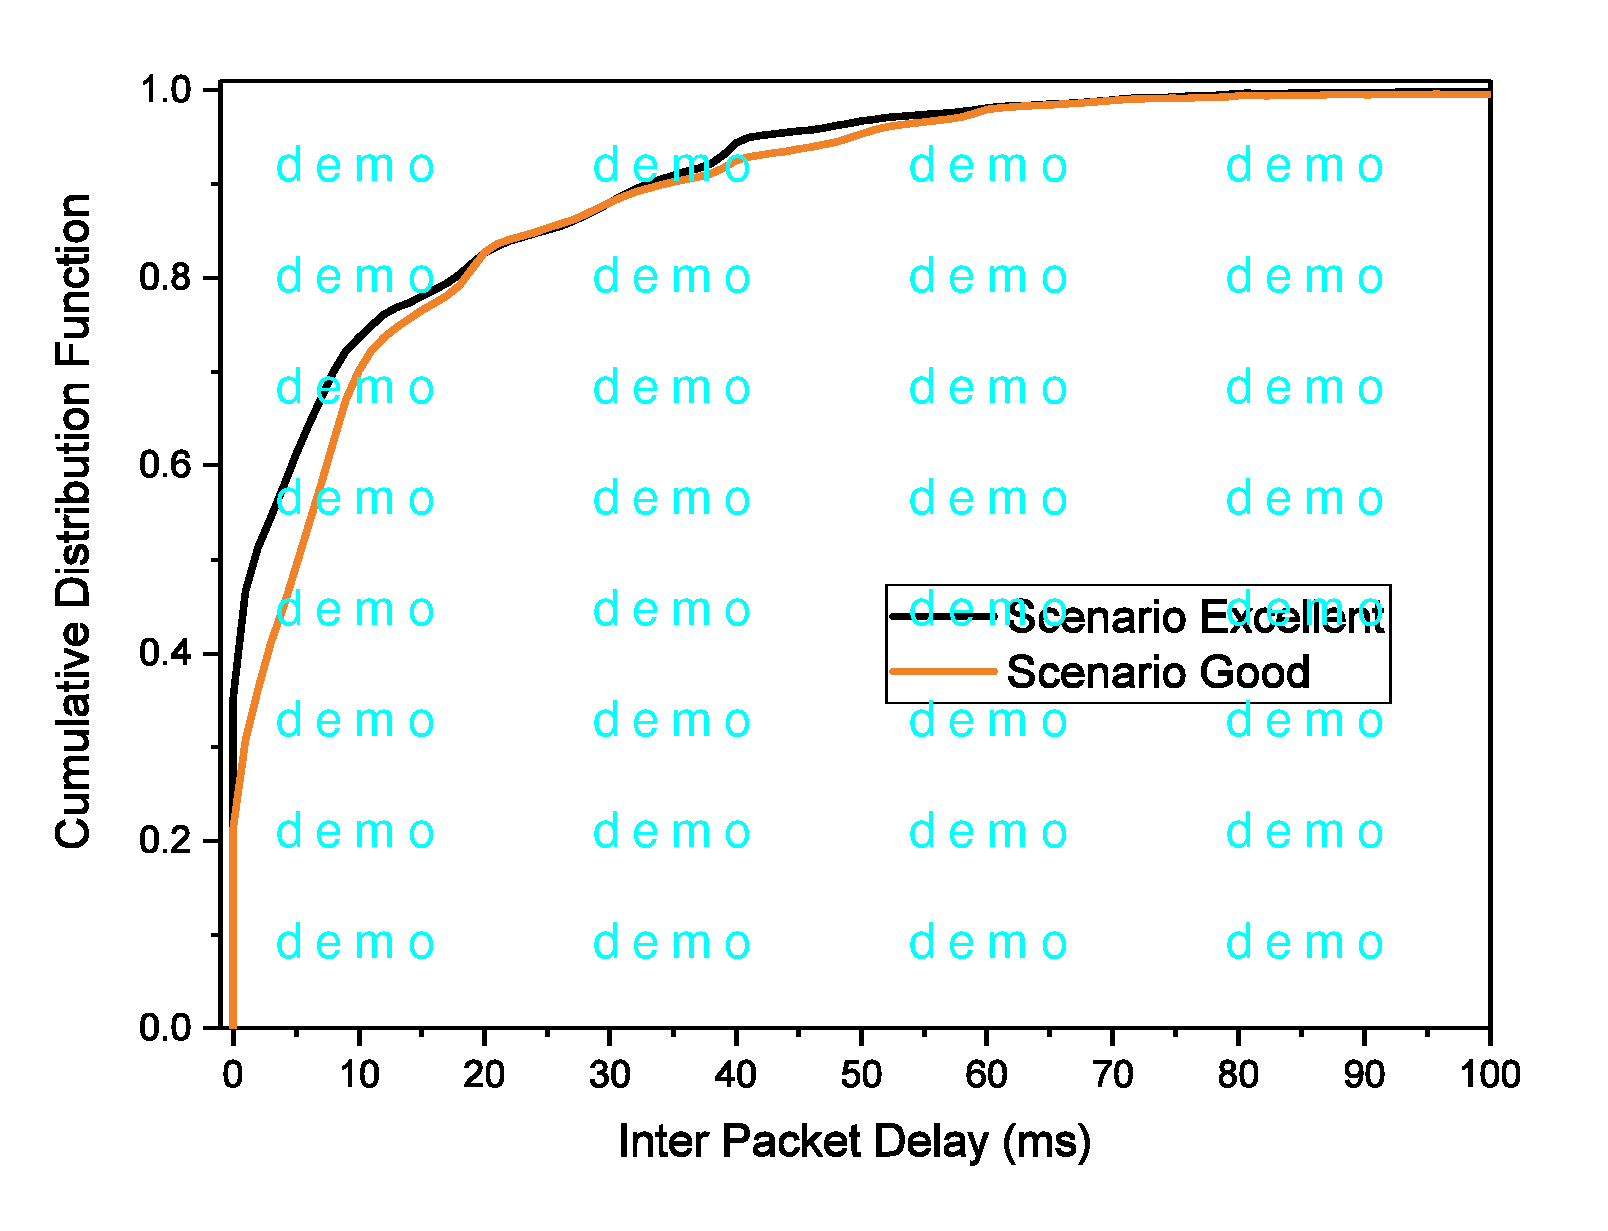
\includegraphics[width=0.48\textwidth]{chapters/chapter3/figures/capture-ipd-cdf.pdf}
        }
        \subfigure[IPD分布的概率质量函数图]{
            \label{fig:3:capture:ipd:pmf}
            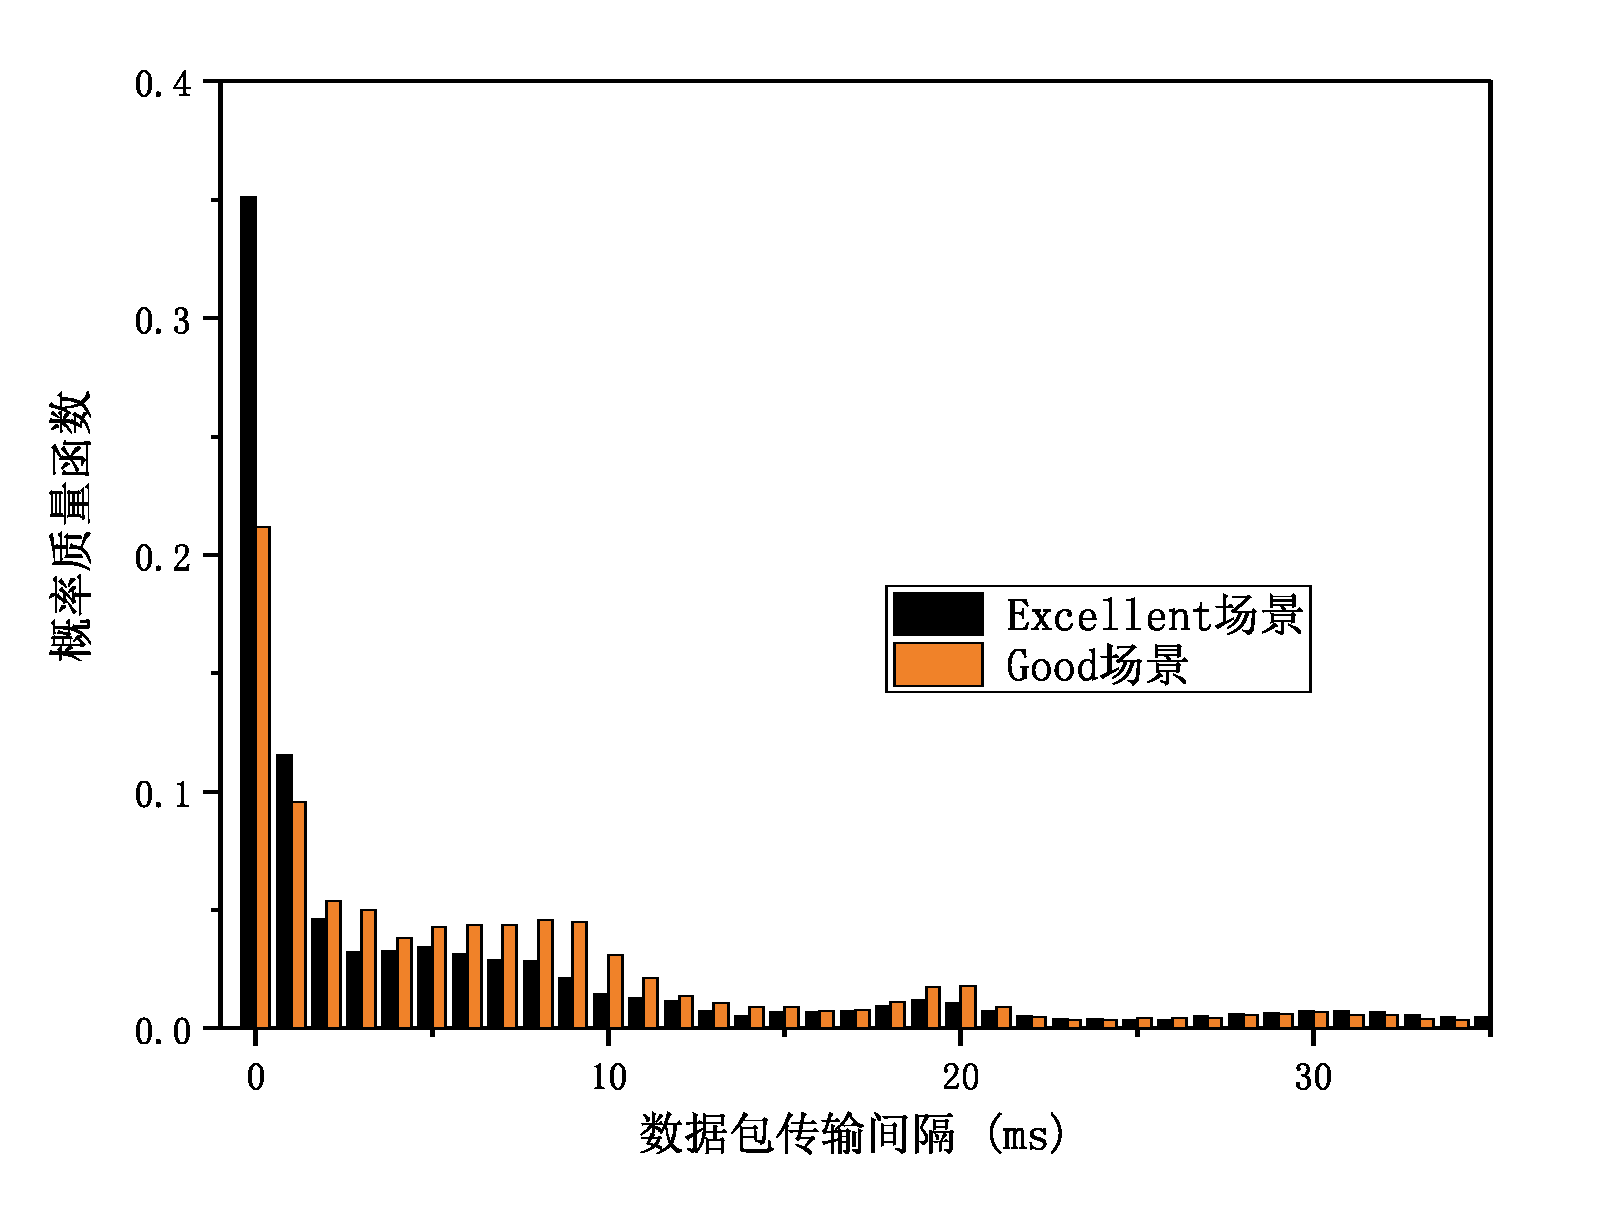
\includegraphics[width=0.48\textwidth]{chapters/chapter3/figures/capture-ipd-pmf.pdf}
        }
    \caption{VoLTE视频数据包IPD分布图}
    \label{fig:3:capture:ipd}
    \end{figure}
}

图\nref{fig:3:capture:ipd}中,分别展示了两种场景下的IPD分布情况。如图\nref{fig:3:capture:ipd:cdf},两种场景中的趋势及数值范围均近似,证明丢包事件对IPD总体分布不明显。图\nref{fig:3:capture:ipd:pmf}中,IPD的概率质量函数在不同场景中也具有近似的趋势。综合概率质量函数及累积分布函数的变化趋势,对于基于主动丢包的时间隐通道,仅通过IPD分布进行检测是不完善的。另一方面,证明了基于主动丢包的时间隐通道构建方法,在当前检测方法面前具有较好的隐蔽性。

\subsection{突发丢包长度}
\label{chap:analyze:results:burst}

%什么是突发丢包长度
网络中的丢包事件,通常分为随机丢包和一定长度的突发丢包,随机丢包为单个数据包随机丢失,突发丢包为多个数据包连续丢失。\nupcite{816237,6711984}。对于与基于VoIP的视频通话来说,随机丢包持续影响视频质量,突发丢包主要影响通话稳定性。\nupcite{5977359,6894614,1709847}本文中,将随机丢包作为突发丢包的一种特征情况,即长度为1的突发丢包,在分布统计中统一处理。

%两种场景下,测试得到的突发丢包长度信息
\insertFigure{
    \begin{figure}[htbp]
        \centering
            \subfigure[突发丢包长度的累积分布函数图]{
                \label{fig:3:capture:burst:cdf}
                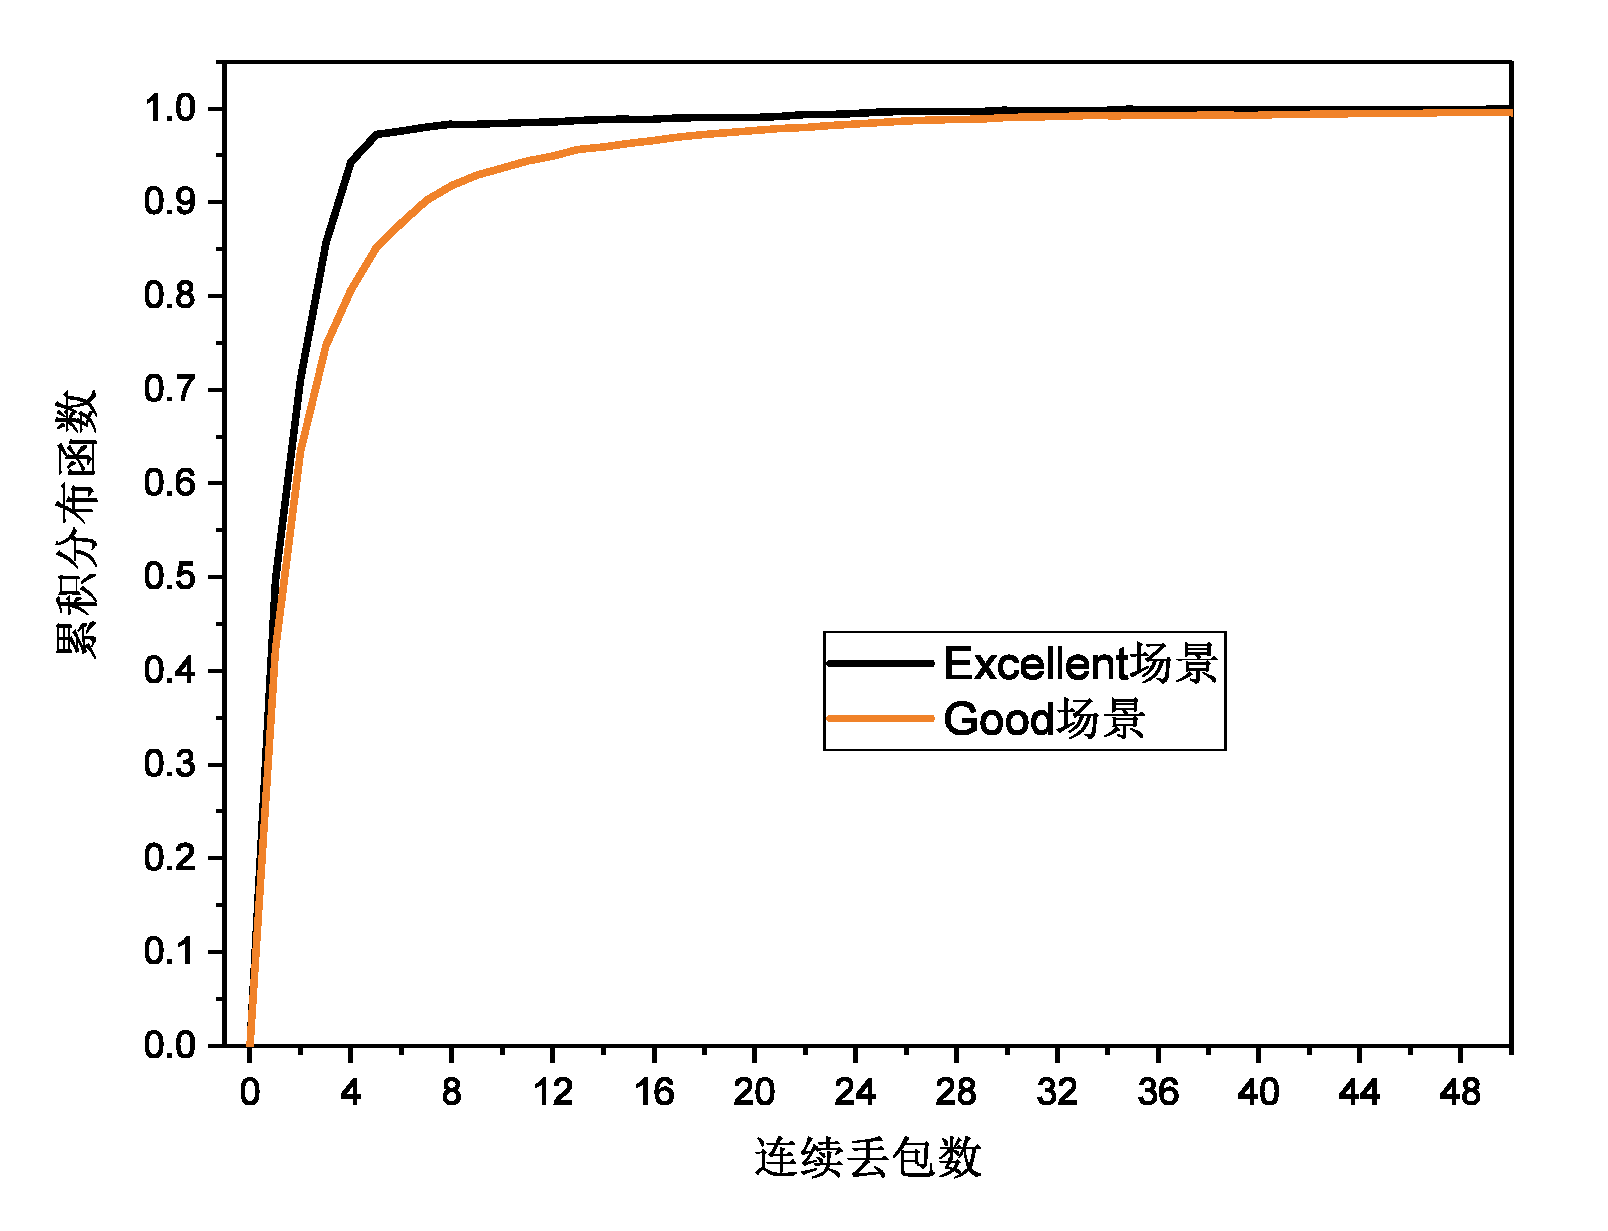
\includegraphics[width=0.48\textwidth]{chapters/chapter3/figures/capture-cdf-burst.pdf}
            }
            \subfigure[突发丢包长度的概率质量函数图]{
                \label{fig:3:capture:burst:pmf}
                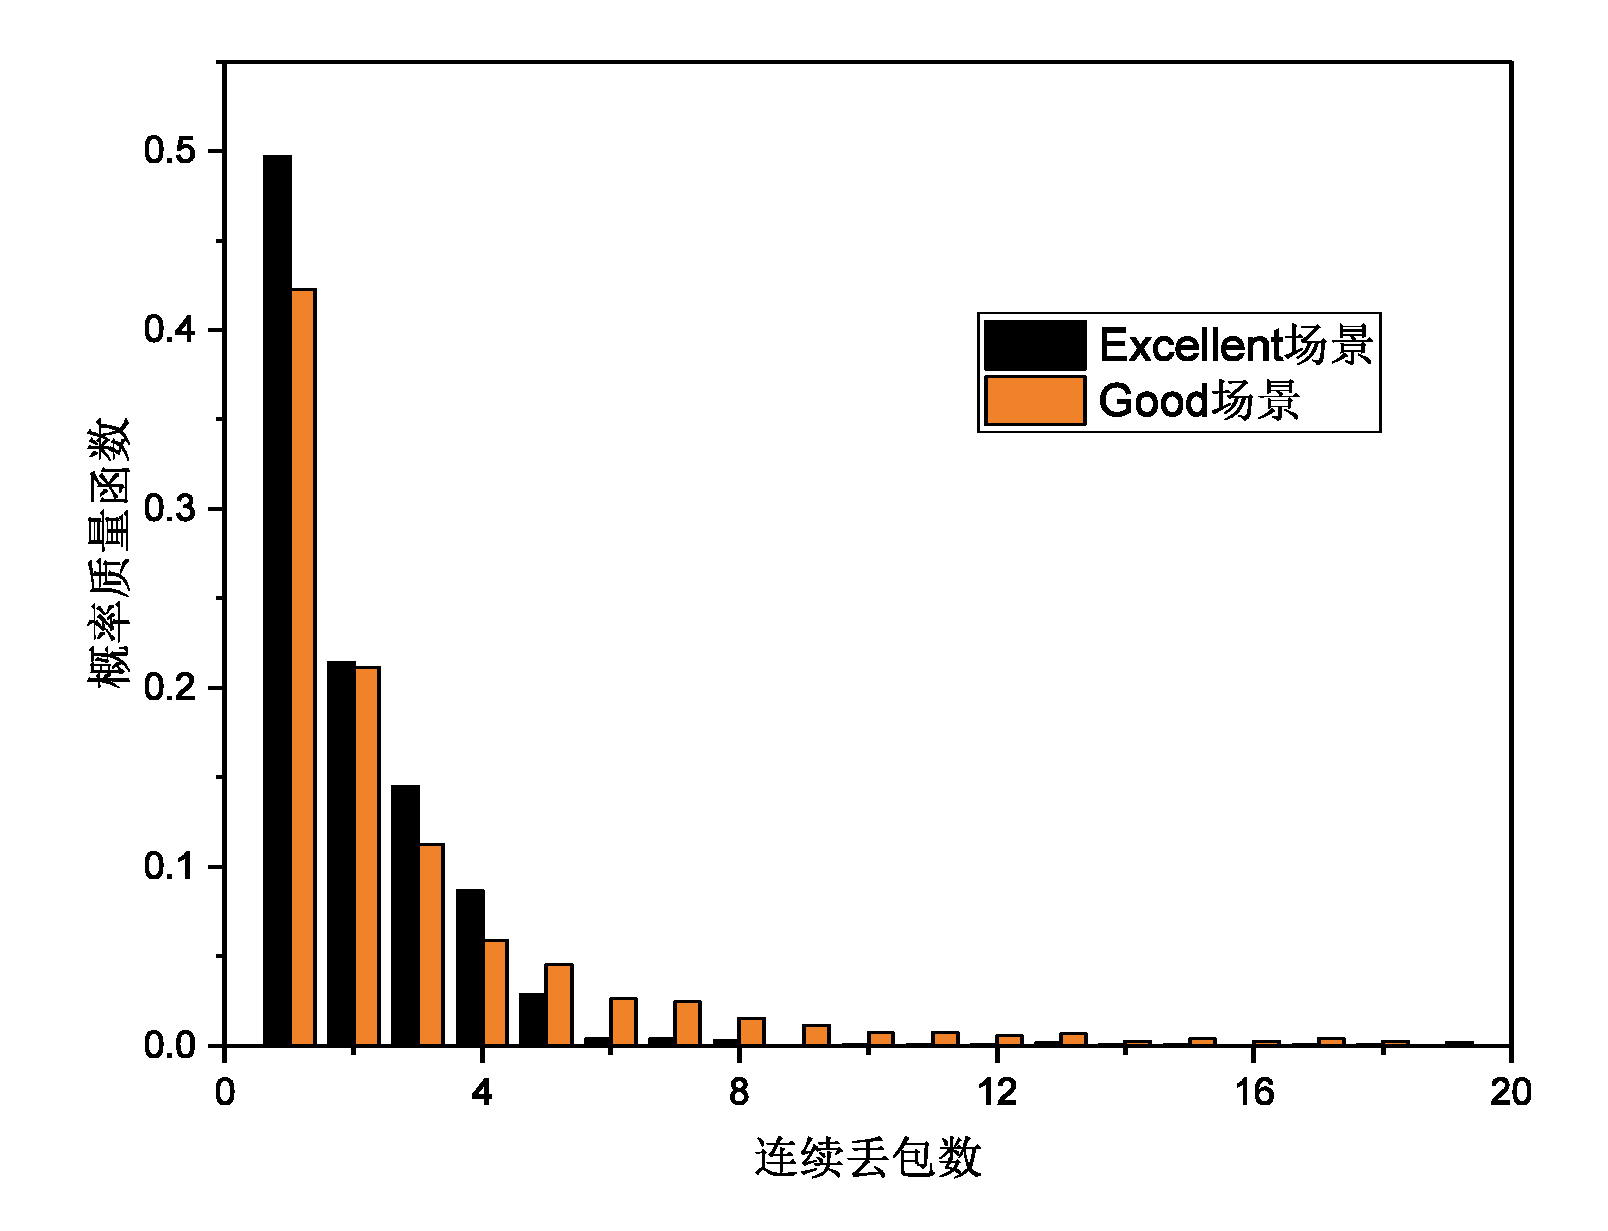
\includegraphics[width=0.48\textwidth]{chapters/chapter3/figures/capture-pmf-burst.pdf}
            }
        \caption{两种场景中突发丢包长度的分布图}
        \label{fig:3:capture:burst}
    \end{figure}
}

如图\nref{fig:3:capture:burst},在两种网络场景中,突发长度的分布趋势趋于一致。具体到部分特征,Excellent场景与Good场景在突发丢包长度大于1的部分,在总体中的占比存在差异。如图\nref{fig:3:capture:burst:cdf},Excellent场景中,突发丢包长度普遍较小,累积分布函数曲线在起始阶段上升迅速。如图\nref{fig:3:capture:burst:pmf},对于Good场景,连续丢包导致CDF曲线趋近1的速度减缓。基于主动丢包的时间隐通道,导致长度为1的突发丢包增多,一定程度上影响分布曲线。